\documentclass[11pt]{article}
\usepackage{amsmath}
\usepackage{graphicx}
\usepackage{geometry}
\usepackage[hidelinks]{hyperref}
\usepackage{titlesec}
\usepackage{subcaption}
\usepackage{listings}
\usepackage{xcolor}

\lstset{
  basicstyle=\ttfamily\footnotesize,
  keywordstyle=\color{blue},
  commentstyle=\color{gray},
  numbers=left,
  numberstyle=\tiny,
  breaklines=true,
  frame=single,
  tabsize=4
}

\geometry{margin=1in}
\titleformat{\section}{\normalfont\Large\bfseries}{\thesection}{1em}{}
\titleformat{\subsection}{\normalfont\large\bfseries}{\thesubsection}{1em}{}

\title{RT-Crypto-Tracker}
\author{Maria Charisi}
\date{September 2025\\ 
\href{https://github.com/mariaxarisi/RT-Crypto-Tracker}{\texttt{Github Repo}}}

\begin{document}

\maketitle

\begin{abstract}
This report is part of an assignment for the \textit{Embedded and Real Time Systems} class of the Aristotle University's Electrical and Computer Engineering department, under professor \textit{Nikolaos Pitsianis}.

It presents the software architecture, deployment, and performance of a real-time cryptocurrency analysis system. The system collects trading information for eight different cryptocurrencies and computes key statistics, including moving averages and Pearson correlations, which can be used for future predictions. It is designed to run efficiently on a microcomputer for extended periods, while maintaining low CPU usage and preventing memory leaks.
\end{abstract}

\tableofcontents
\newpage

\section{Introduction}
The cryptocurrency market operates continuously, producing a large volume of trading data across various exchanges. Real-time analysis of this data is essential for identifying market trends, evaluating relationships between different assets, and supporting data-driven trading decisions. This project introduces a real-time cryptocurrency analysis system that collects trade information from the \textit{OKX WebSocket API}. The system focuses on the following cryptocurrency trading pairs:

\begin{table} [h]
    \centering
    \begin{tabular}{cccc}
         BTC-USDT & ADA-USDT & SOL-USDT & LTC-USDT\\
         DOGE-USDT & ETH-USDT & XRP-USDT & BNB-USDT\\
    \end{tabular}
    \label{tab:trading_pairs}
\end{table}

The collected trade data are processed to compute statistical measures such as moving averages and Pearson correlations, which provide insights into price trends and interdependencies among cryptocurrencies. The system is designed to run efficiently on low-power microcomputers, allowing continuous operation for days or even weeks with minimal CPU usage.

\section{System Architecture}

The system architecture uses multithreading to ensure efficient, real-time processing of cryptocurrency trading data while maintaining low computational overhead. A total of five dedicated threads are employed, each responsible for a specific task within the pipeline. The \textbf{WebSocket thread} manages the connection to the OKX WebSocket, including reconnection handling and message retrieval. The \textbf{Parser thread} processes incoming messages, extracting relevant trade information. Two computational threads handle statistical analysis: the \textbf{Moving Average thread}, which calculates moving averages for each trading pair, and the \textbf{Pearson thread}, which computes Pearson correlations across symbols. Finally, a \textbf{CPU monitoring thread} tracks resource usage, providing performance statistics.

\subsection{WebSocket Thread}

The WebSocket thread is responsible for establishing and maintaining the connection with the OKX WebSocket server. In the event of a connection error, the thread automatically attempts to reconnect every two seconds to ensure continuous data acquisition. Additionally, if the user signals the program to terminate, this thread gracefully closes the WebSocket connection.  

When a message is received from the server, the WebSocket thread pushes it into a shared message queue. This queue is implemented as a thread-safe structure using a mutex to synchronize access and a \texttt{not\_empty} condition variable to notify the parser thread when new data is available. This design ensures reliable message passing between the WebSocket thread and the parser thread without data loss or race conditions.

\subsection{Parser Thread}

The parser thread is responsible for consuming messages from the message queue described earlier. Each message contains trade information received from the WebSocket connection. The parser extracts relevant fields such as the timestamp, price, and trade size, and encapsulates them in a \texttt{Trade} structure:
\begin{lstlisting}[language=C]
typedef struct Trade {
    long long ts;   // trade timestamp
    double px;      // trade price
    double sz;      // trade size
} Trade;
\end{lstlisting}

Once a \texttt{Trade} instance is created, it is appended to the corresponding trade vector associated with its trading pair. To ensure thread safety and prevent race conditions, these trade vectors are protected by mutexes, allowing multiple threads to operate on the data structures concurrently.

\subsection{Moving Average Thread}

The moving average thread is initialized with a start time provided by the main function. This timestamp is rounded up to the next full minute, which becomes the baseline for the calculations. From then on, the thread waits until each successive full minute before performing its computations. This ensures that moving averages for all symbols are calculated at consistent, minute-aligned intervals.

\begin{lstlisting}[language=C]
void* average_thread_func(void *arg) {
    long long base_time = *(long long *)arg;
    base_time = base_time - (base_time % ONE_MINUTE_MS) + ONE_MINUTE_MS;

    while (!interrupted) {
        long long now = current_timestamp_ms();
        if (now < base_time)
            usleep((base_time - now) * 1000);

        for (int i = 0; i < SYMBOL_COUNT; i++)
            calculate_moving_average(i, base_time);

        base_time += ONE_MINUTE_MS;
    }
    return NULL;
}
\end{lstlisting}

At each cycle, the thread calculates a 15-minute volume-weighted moving average for every trading pair. The calculation window spans from the current minute (\texttt{window\_end}) back to 15 minutes earlier (\texttt{window\_start}). For each trade stored in the corresponding trade vector, trades older than the window are discarded, while those within the window contribute to the summation of \texttt{price $\times$ size} and total traded volume. The moving average is then computed as:

\[
\text{mv\_average} = \frac{\sum (price \times size)}{\sum size}
\]

and stored in a \texttt{MvAverage} structure:

\begin{lstlisting}[language=C]
typedef struct MvAverage {
    long long ts;    // timestamp of the average
    double value;    // computed average value
} MvAverage;
\end{lstlisting}

Each \texttt{MvAverage} instance is appended to a dedicated cyclic buffer for the corresponding symbol, making the data available for later correlation analysis.

While functional, the current use of trade vectors introduces overhead when removing outdated trades, since erasing elements at the beginning of a vector requires shifting all subsequent elements. This limitation is reflected in performance measurements, as we can observe in Figure~\ref{fig:mv-delay}. A more efficient solution would be to employ a cyclic buffer with dynamic size management, thereby avoiding costly element shifts and reducing computational overhead.

\subsection{Pearson Correlation Thread}
The Pearson correlation thread is responsible for quantifying relationships between trading pairs based on their recent moving averages. Its execution flow is similar to the moving average thread: it is initialized with a start time, aligned to the next full minute, and then iterates once per minute until interrupted. To ensure enough data is available, the thread begins its calculations only after the first eight minutes of operation.

For each trading pair, the thread determines the maximum Pearson correlation with all other pairs over the past hour. The calculation is performed by comparing the most recent eight moving averages of the target symbol against every sequential set of eight moving averages from the other symbols. To support this rolling computation efficiently, moving averages are stored in cyclic buffers with a capacity of 67 entries (corresponding to one hour plus additional overlap). The result with the highest correlation value is recorded and written to the system logs for later analysis.

The correlation itself is computed using the standard Pearson formula:

\[
pearson\_corr = \frac{\sum (x_i y_i) - \frac{\sum x_i \sum y_i}{n}}
{\sqrt{\Big(\sum x_i^2 - \frac{(\sum x_i)^2}{n}\Big) \Big(\sum y_i^2 - \frac{(\sum y_i)^2}{n}\Big)}}
\]

\section{Compilation and Deployment}

The build system is implemented using a \texttt{Makefile}, which supports both native compilation on the host machine and cross-compilation for deployment on a Raspberry Pi device.

\subsection{Native Compilation}
For development on the host system, the project uses the GNU Compiler Collection (\texttt{gcc}). The default build can be invoked with:

\begin{lstlisting}[language=bash]
make
\end{lstlisting}

This compiles all source files into object files under \texttt{obj/} and links them into the executable \texttt{crypto}. The build links against external libraries including \texttt{jansson}, \texttt{libwebsockets}, and \texttt{pthread}.

\subsection{Cross Compilation for Raspberry Pi}
To target a Raspberry Pi, the Makefile provides a dedicated build rule \texttt{make pi}, which uses the ARM cross-compiler \texttt{arm-linux-gnueabihf-gcc}. A sysroot is required to mirror the Raspberry Pi’s filesystem, providing the correct headers and libraries. In this setup, the sysroot is located under:

\begin{lstlisting}[language=bash]
$(HOME)/rpi-sysroot
\end{lstlisting}

Cross-compilation is invoked with:

\begin{lstlisting}[language=bash]
make pi
\end{lstlisting}

This produces the binary \texttt{crypto-pi}, with its object files placed in \texttt{obj-pi/}. The resulting executable is linked against the Raspberry Pi’s versions of \texttt{libssl}, \texttt{libcrypto}, \texttt{libwebsockets}, ensuring compatibility.

\section{Results}

The system was deployed on a Raspberry Pi Zero 2 W using a cross-compiled executable, which ran continuously for three days to collect performance and correlation data.

\subsection{Performance Statistics}

Figures~\ref{fig:mv-delay} and~\ref{fig:pearson-delay} illustrate the per-minute delays of the moving average and Pearson correlation threads, respectively. Across all three days, both threads complete their computations within the one-minute interval, ensuring no overlap into the next cycle.  

The Pearson thread exhibits excellent performance, with delays consistently below 0.12 seconds. The moving average thread is mostly efficient, but occasional spikes reach up to 30 seconds. These spikes are caused by the overhead of removing outdated trades from the vectors used to store trade data. Despite this, the thread never exceeds the one-minute limit, maintaining accurate and timely calculations.

\begin{figure}[h]
    \centering
    \begin{subfigure}{0.48\textwidth}
        \centering
        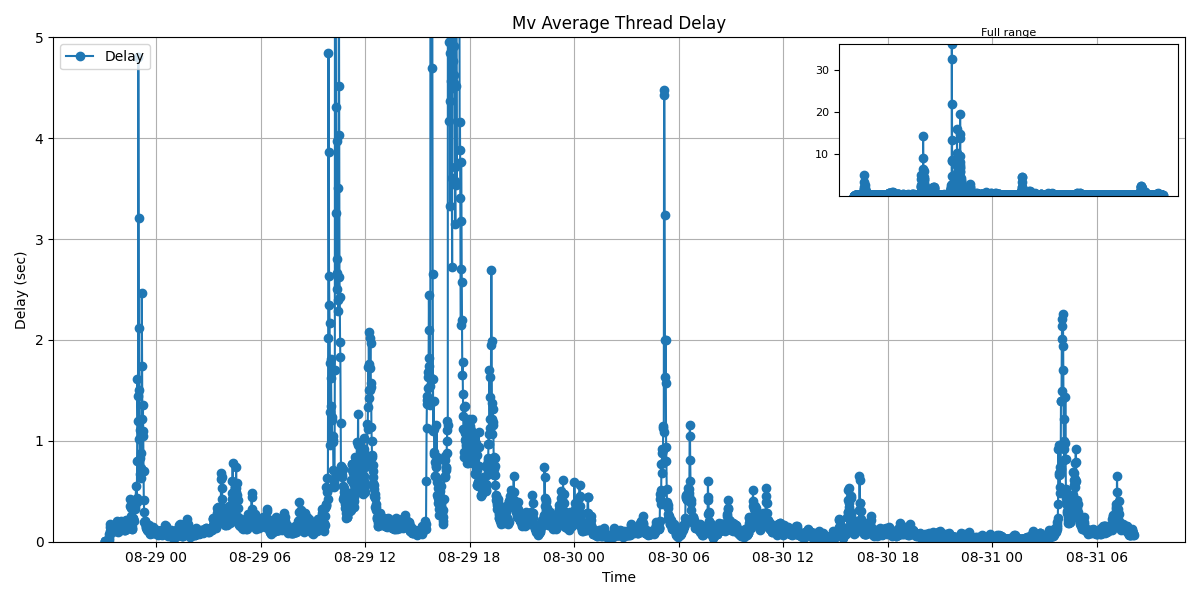
\includegraphics[width=\linewidth]{../assets/mv-average-thread-delay.png}
        \caption{}
        \label{fig:mv-delay}
    \end{subfigure}
    \hfill
    \begin{subfigure}{0.48\textwidth}
        \centering
        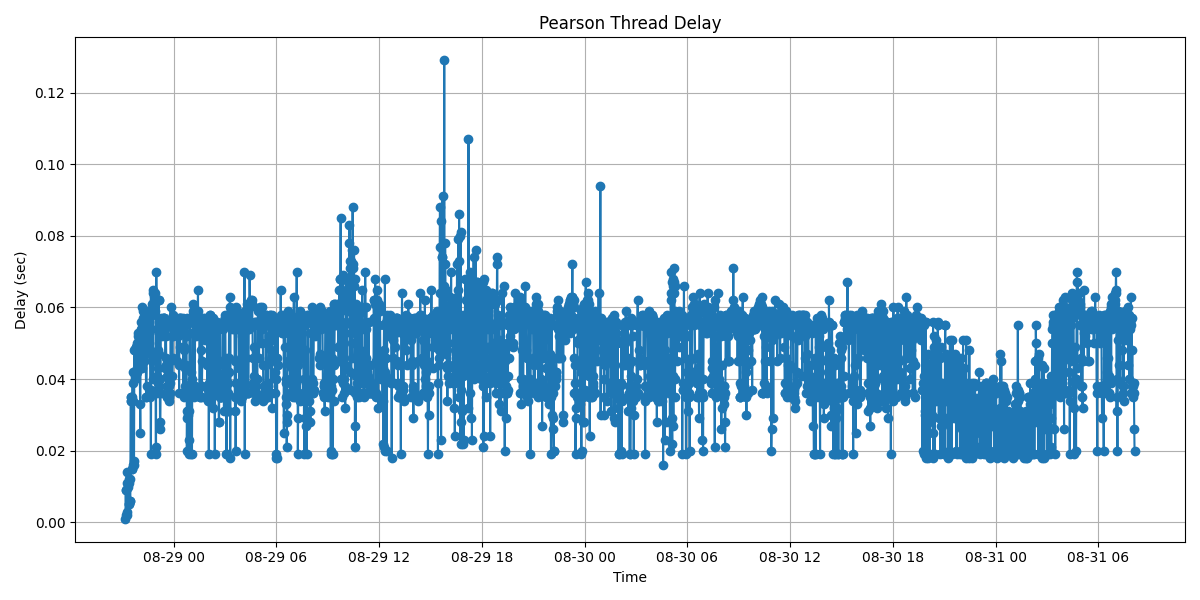
\includegraphics[width=\linewidth]{../assets/pearson-thread-delay.png}
        \caption{}
        \label{fig:pearson-delay}
    \end{subfigure}
    \caption{Thread delays: (a) moving average thread, (b) Pearson correlation thread.}
    \label{fig:thread-delays}
\end{figure}

Figure~\ref{fig:cpu-usage} shows the CPU usage per minute over the three days. In general, the CPU remains around 5\%, demonstrating the low computational load of the system. However, short peaks reaching up to 50\% occur during moments when the moving average thread experiences high delays or when the program reconnects to the WebSocket server.

\begin{figure}[h]
    \centering
    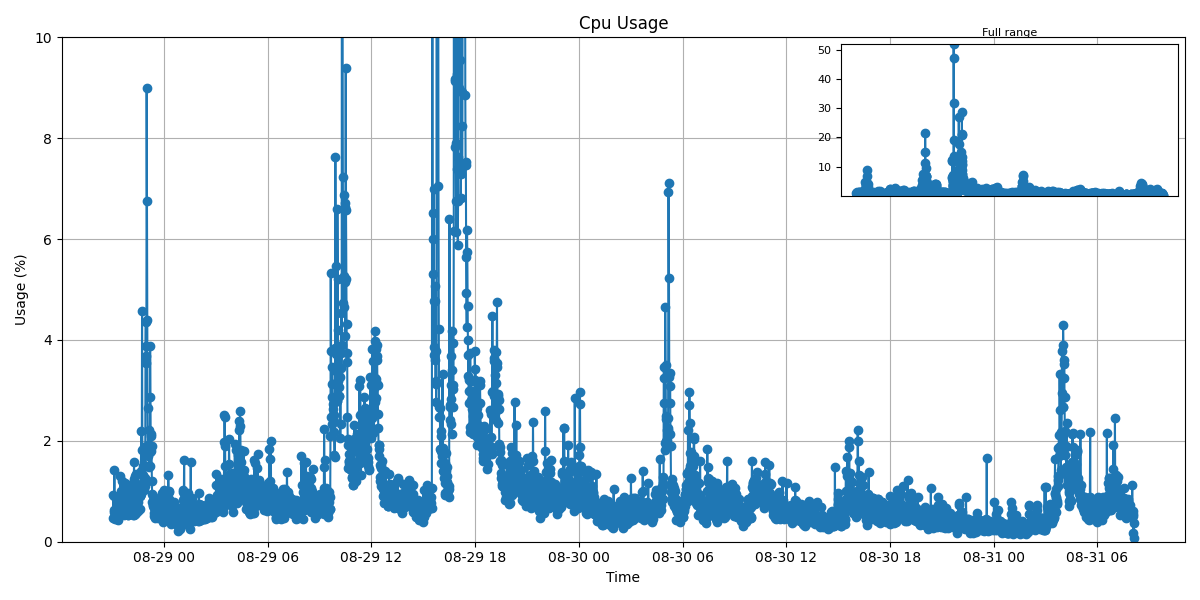
\includegraphics[width=0.7\textwidth]{../assets/CPU-usage.png}
    \caption{CPU usage percentage over time.}
    \label{fig:cpu-usage}
\end{figure}

\subsection{Correlation Analysis}

Figures~\ref{fig:correlations1} and~\ref{fig:correlations2} visualize the maximum correlations over time for each trading pair.
Each plot consists of two elements:

\begin{itemize}
    \item A bar chart where the color of each bar indicates the trading pair with which the current symbol had the maximum correlation at that minute.
    
    \item A black timeline overlaid on the bars that represents the actual correlation value.
\end{itemize}

For clarity, only one day of data is shown, as visualizing the full three-day experiment would have made the plots harder to interpret.

\section{Conclusion}

This report presented the design and evaluation of a real-time cryptocurrency analysis system capable of continuous operation on low-power embedded hardware. By combining a modular multithreaded architecture, efficient synchronization mechanisms, and lightweight statistical computations, the system achieved reliable performance with minimal resource usage. Experimental deployment on a Raspberry Pi Zero 2 W demonstrated that the system can sustain uninterrupted data collection and processing for multiple days.

Future work will explore more advanced statistical models, optimized data structures (e.g., cyclic buffer for trade data), and real-time dashboards for live monitoring. These enhancements will further improve scalability, reduce computational overhead, and extend the system’s applicability to more complex market analysis tasks.

\section{References}

\begin{itemize}
  \item Finnhub WebSocket API: \url{https://finnhub.io/docs/api/websocket-trades}
  \item libwebsockets official documentation: \url{https://libwebsockets.org/}
\end{itemize}

\begin{figure}[p]
    \captionsetup[subfigure]{labelformat=empty}

    \centering
    \begin{subfigure}{\linewidth}
        \centering
        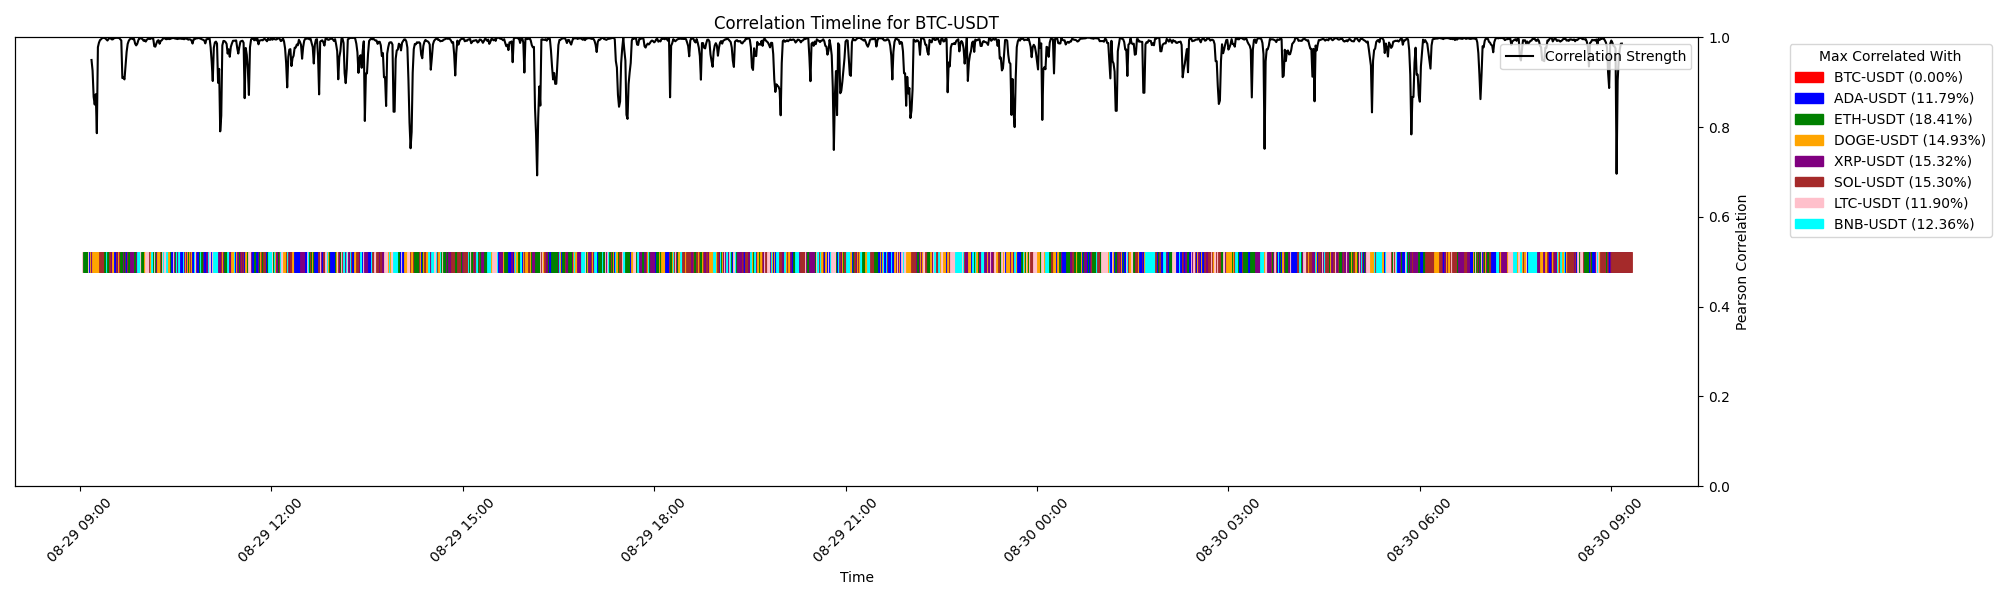
\includegraphics[width=\linewidth]{../assets/correlations/BTC-USDT.png}
        \caption{Maximum correlations over time for BTC-USDT.}
        \label{fig:btc-corr}
    \end{subfigure}

    \vspace{0.1cm}

    \begin{subfigure}{\linewidth}
        \centering
        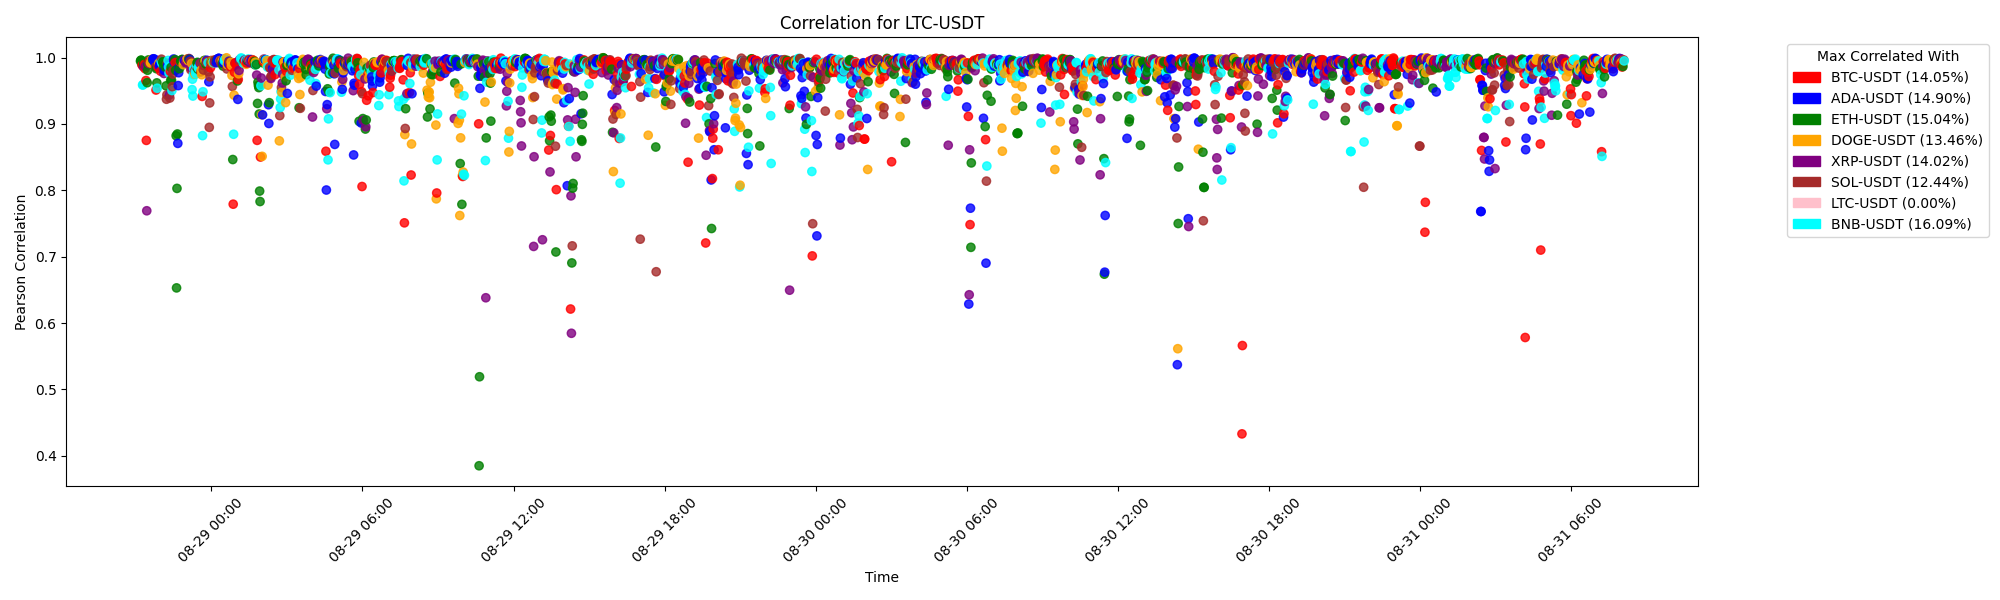
\includegraphics[width=\linewidth]{../assets/correlations/LTC-USDT.png}
        \caption{Maximum correlations over time for LTC-USDT.}
        \label{fig:ltc-corr}
    \end{subfigure}

    \vspace{0.1cm}

    \begin{subfigure}{\linewidth}
        \centering
        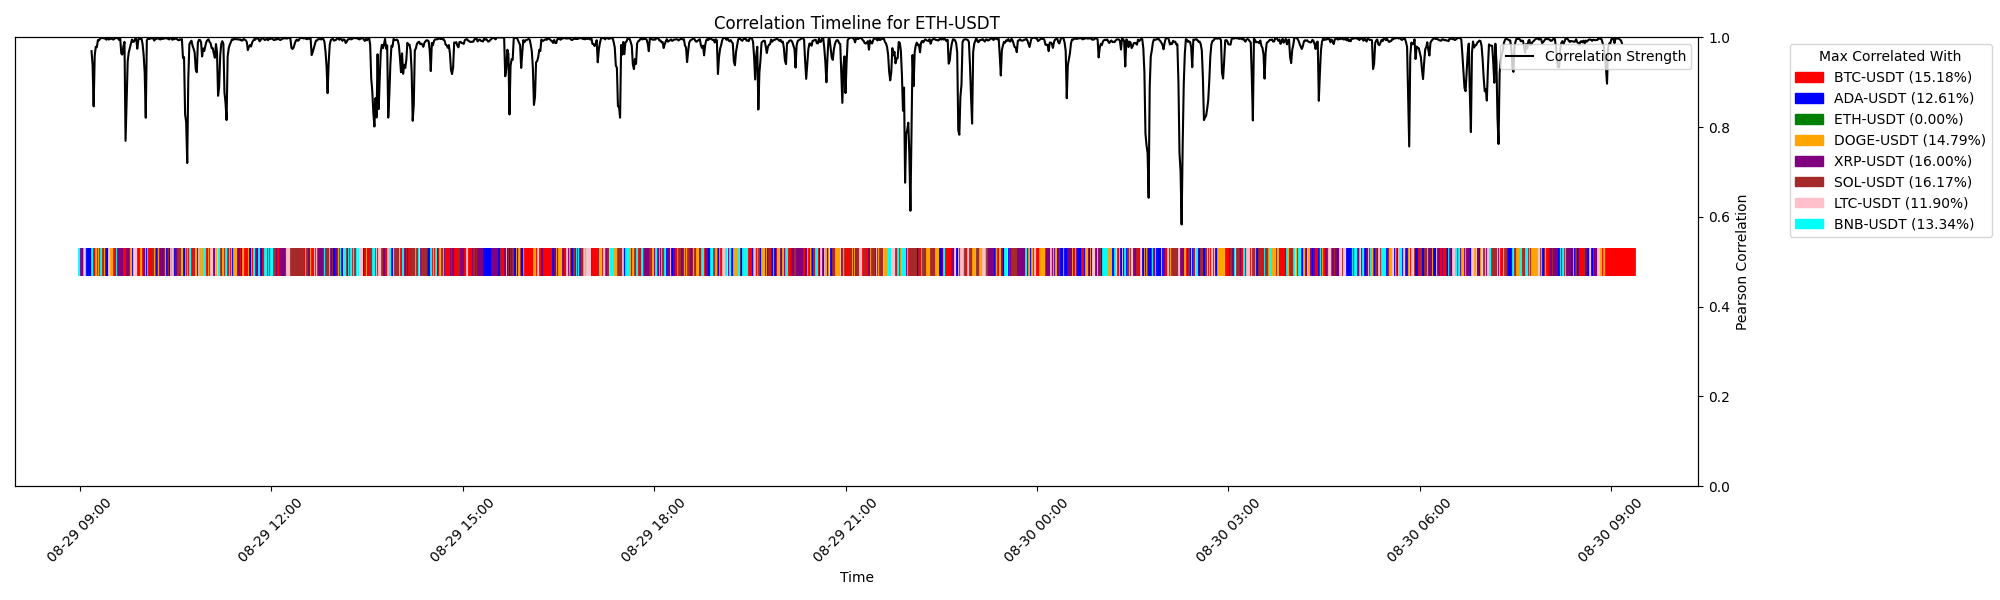
\includegraphics[width=\linewidth]{../assets/correlations/ETH-USDT.png}
        \caption{Maximum correlations over time for ETH-USDT.}
        \label{fig:eth-corr}
    \end{subfigure}

    \vspace{0.1cm}

    \begin{subfigure}{\linewidth}
        \centering
        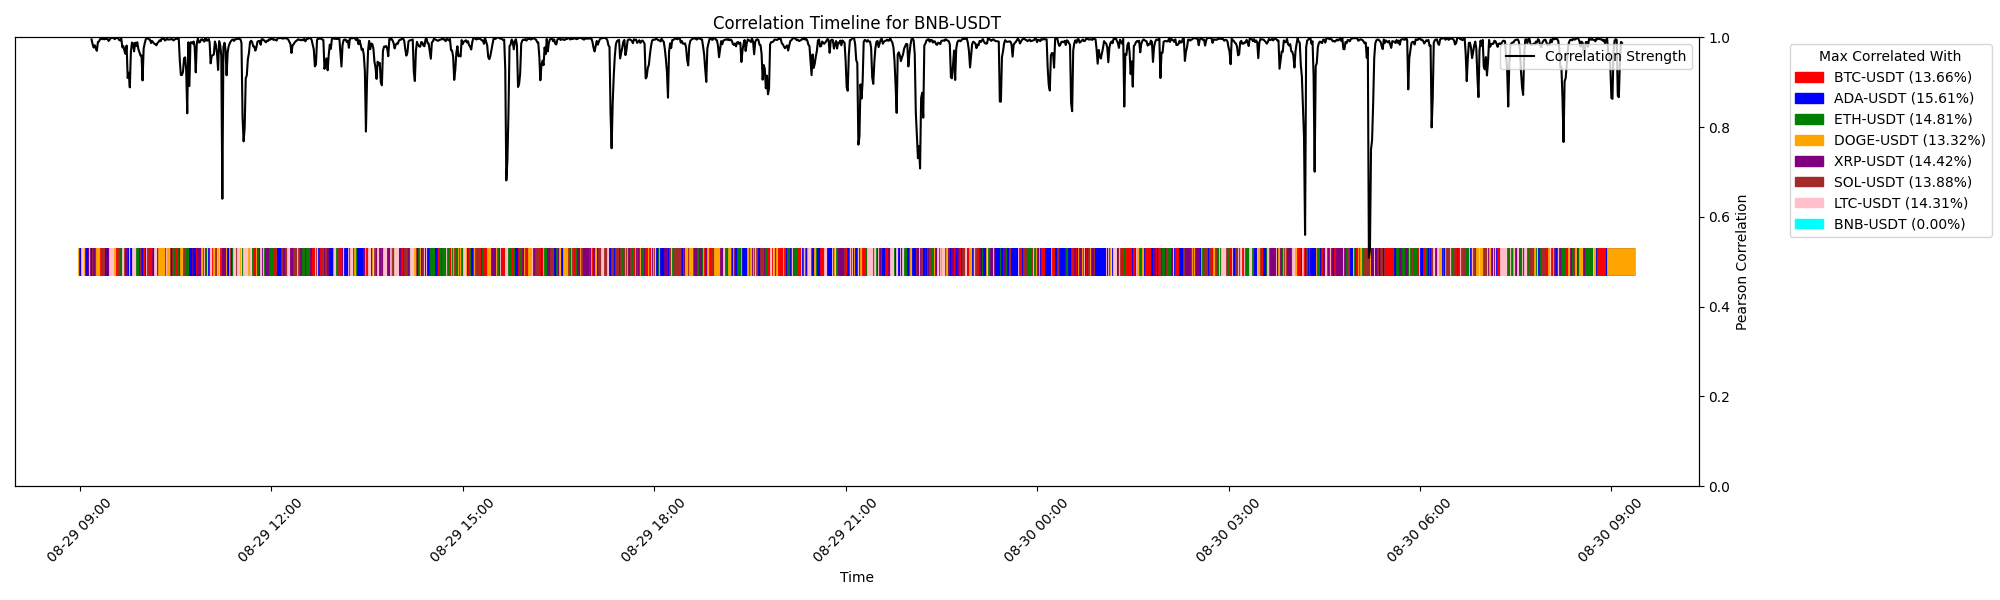
\includegraphics[width=\linewidth]{../assets/correlations/BNB-USDT.png}
        \caption{Maximum correlations over time for BNB-USDT.}
        \label{fig:bnb-corr}
    \end{subfigure}
    \caption{}
    \label{fig:correlations1}
\end{figure}

\begin{figure}[p]
    \captionsetup[subfigure]{labelformat=empty}
    \centering
    \begin{subfigure}{\linewidth}
        \centering
        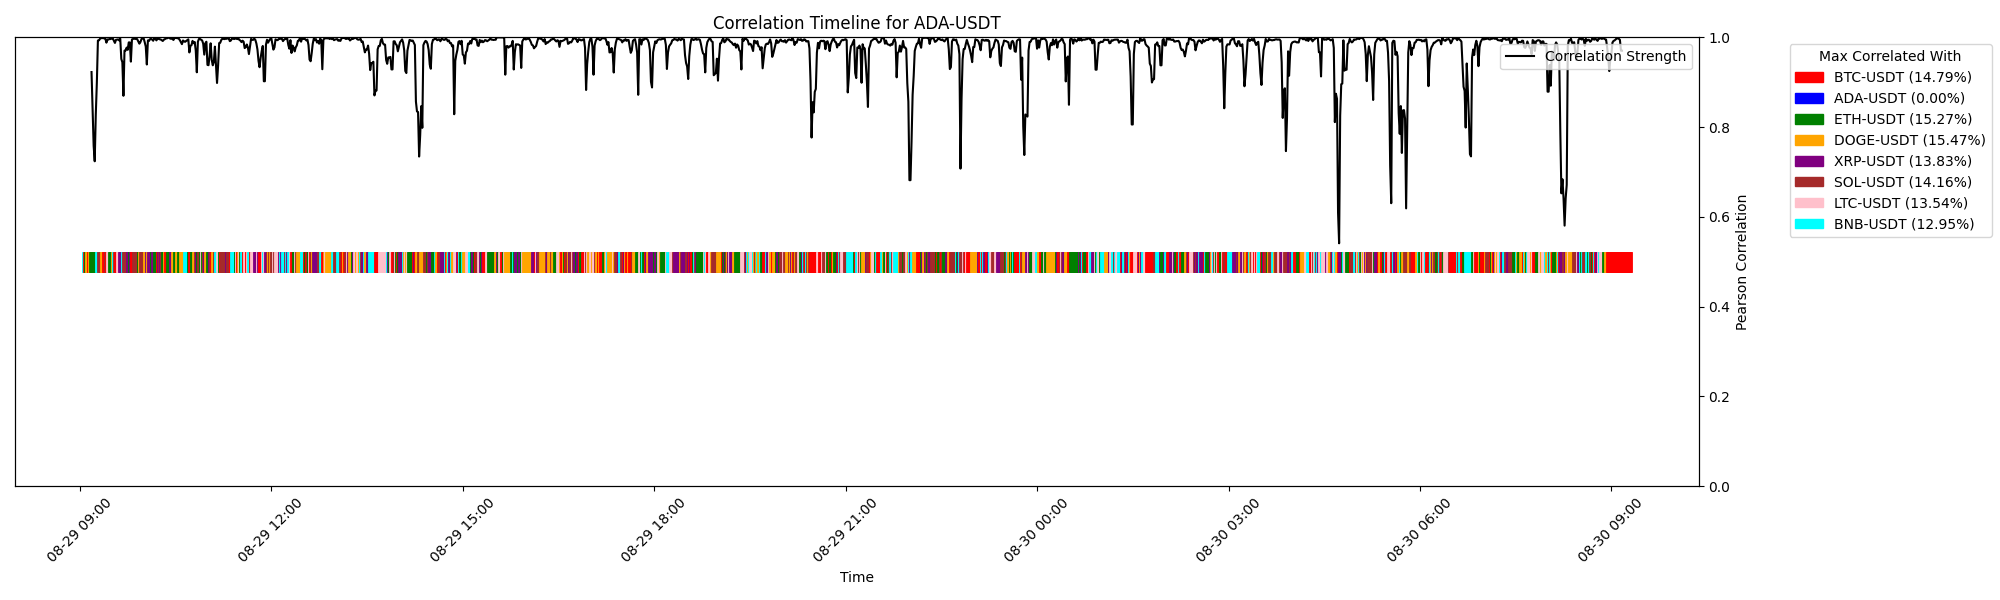
\includegraphics[width=\linewidth]{../assets/correlations/ADA-USDT.png}
        \caption{Maximum correlations over time for ADA-USDT.}
        \label{fig:ada-corr}
    \end{subfigure}

    \vspace{0.1cm}

    \begin{subfigure}{\linewidth}
        \centering
        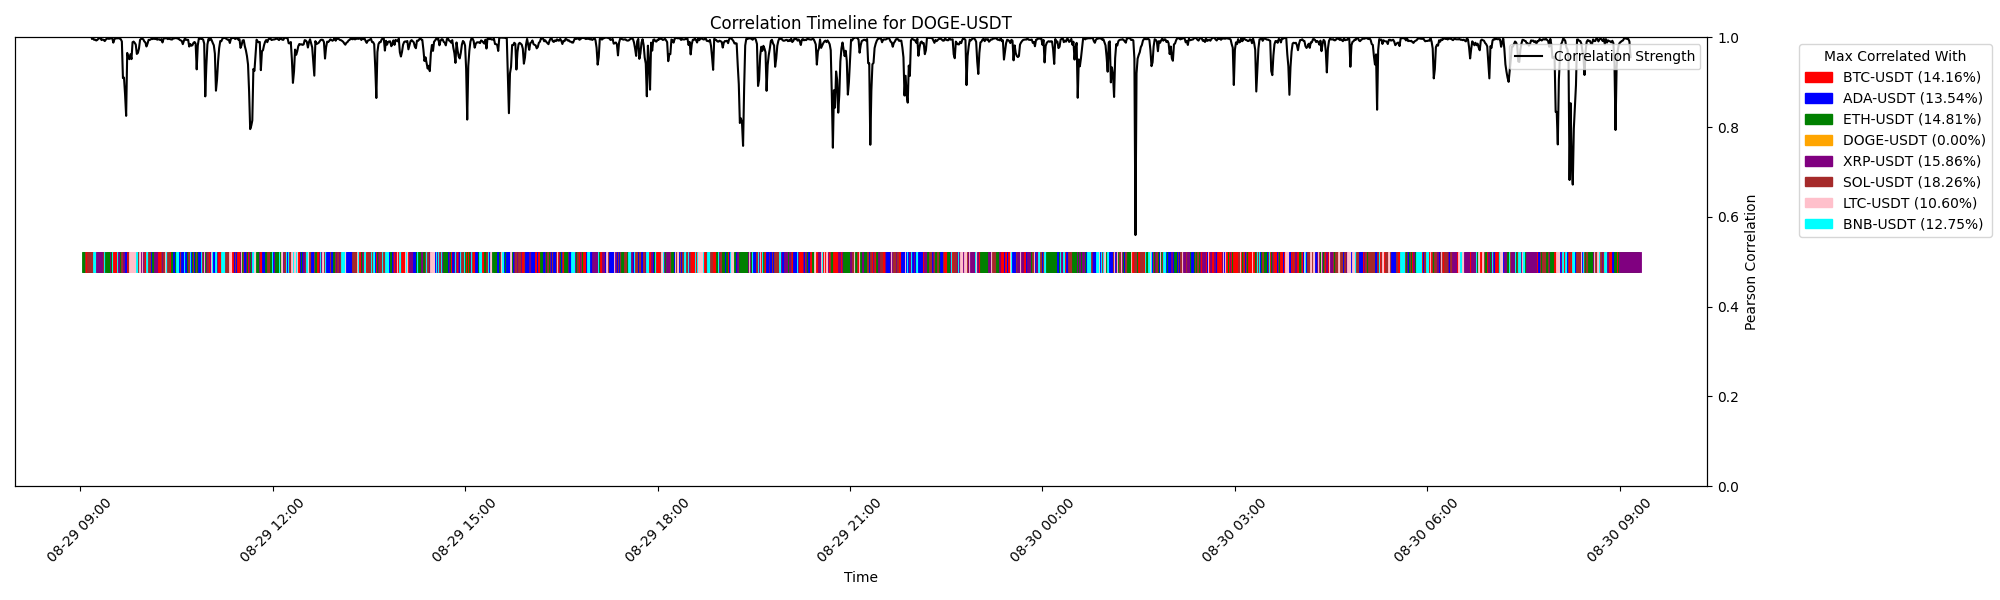
\includegraphics[width=\linewidth]{../assets/correlations/DOGE-USDT.png}
        \caption{Maximum correlations over time for DOGE-USDT.}
        \label{fig:doge-corr}
    \end{subfigure}

    \vspace{0.1cm}

    \begin{subfigure}{\linewidth}
        \centering
        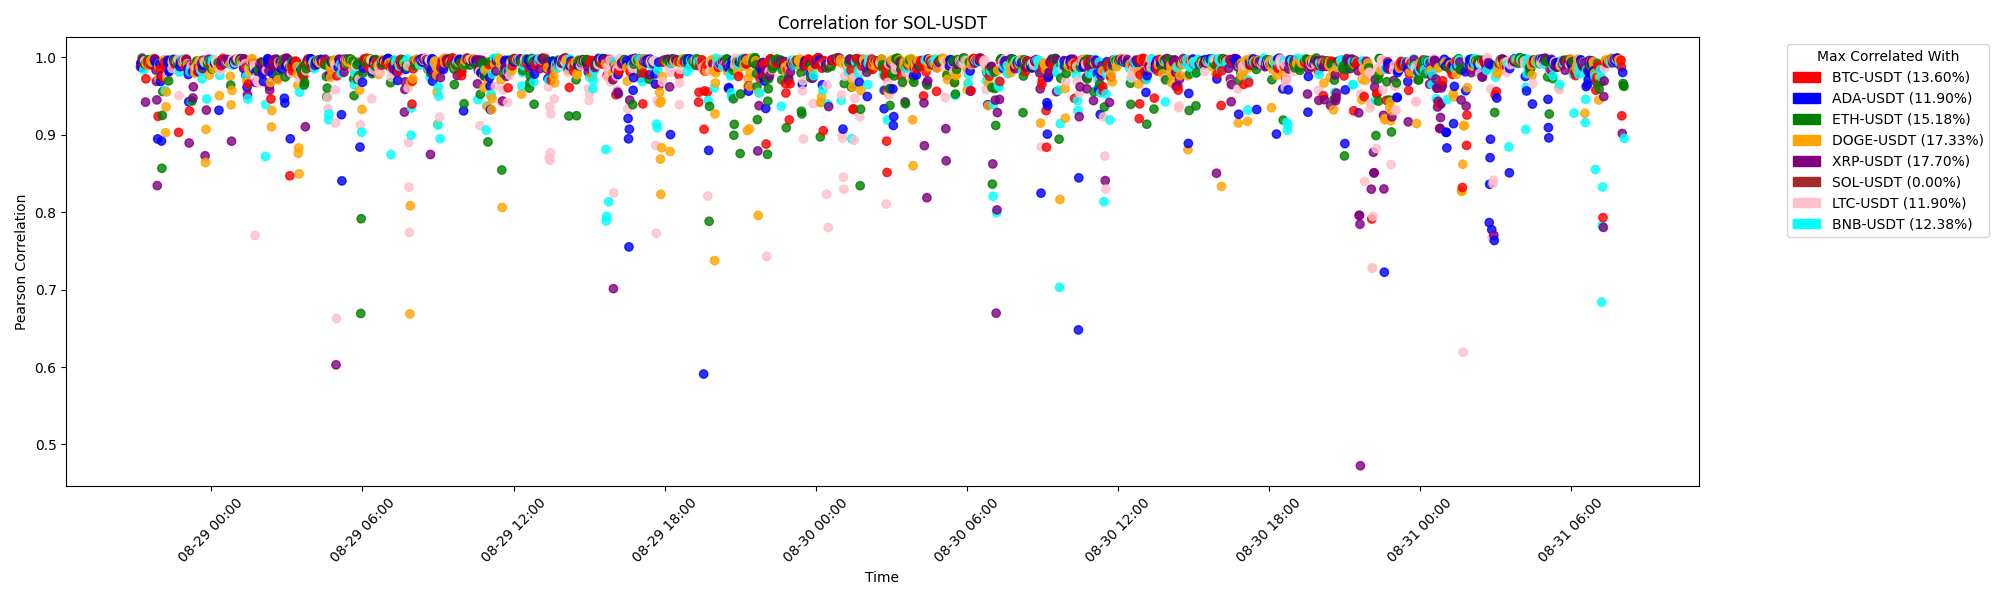
\includegraphics[width=\linewidth]{../assets/correlations/SOL-USDT.png}
        \caption{Maximum correlations over time for SOL-USDT.}
        \label{fig:sol-corr}
    \end{subfigure}

    \vspace{0.1cm}

    \begin{subfigure}{\linewidth}
        \centering
        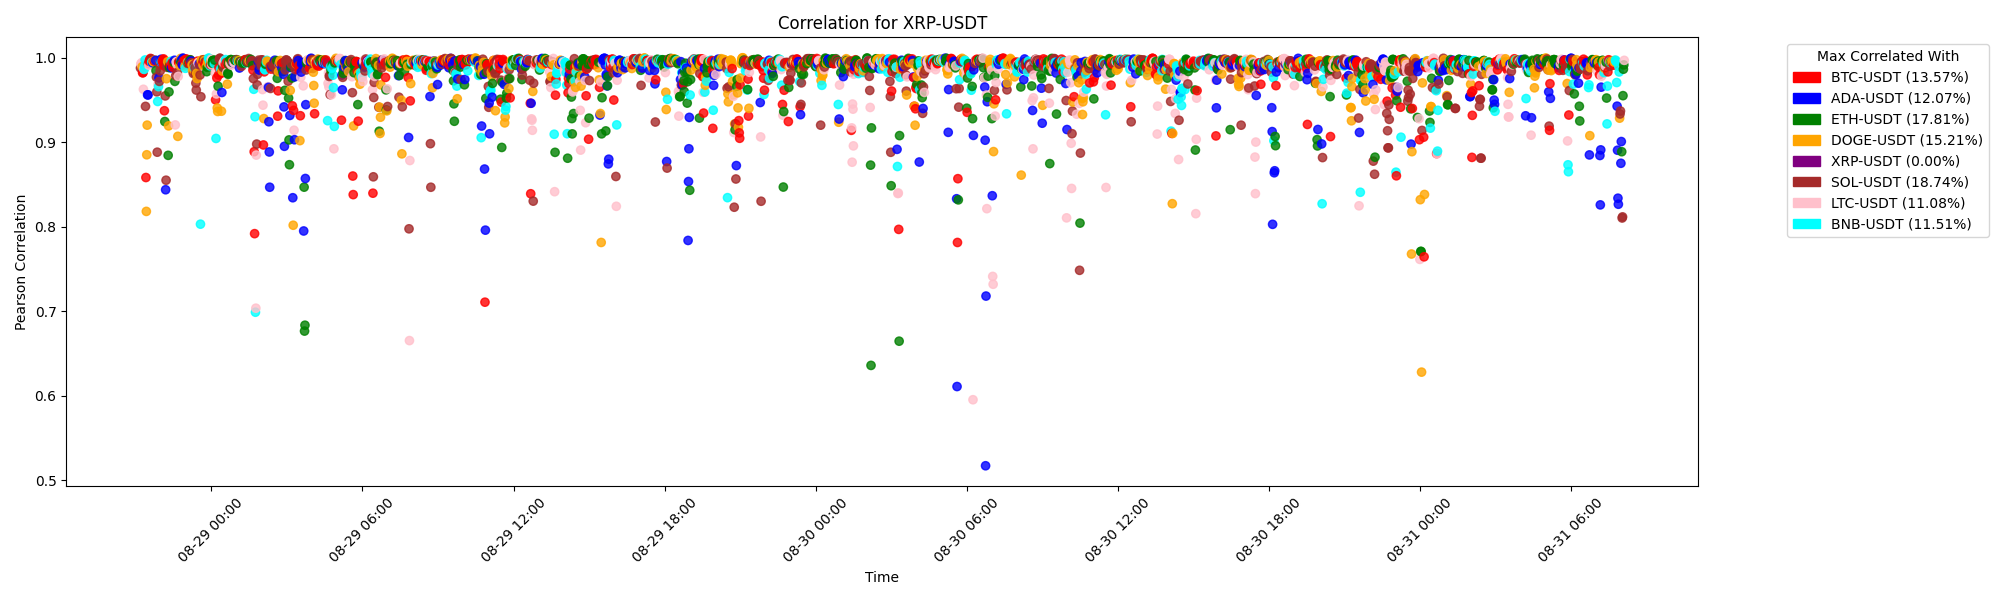
\includegraphics[width=\linewidth]{../assets/correlations/XRP-USDT.png}
        \caption{Maximum correlations over time for XRP-USDT.}
        \label{fig:xrp-corr}
    \end{subfigure}
    \caption{}
    \label{fig:correlations2}
\end{figure}

\end{document}
